% xelatex
% chktex-file 1
% chktex-file 8
% chktex-file 13
% chktex-file 24
% chktex-file 36

\documentclass[10pt]{article}
\usepackage[top=20mm,bottom=20mm,left=20mm,right=20mm]{geometry}

\usepackage{xeCJK}
\usepackage{ctex}

\usepackage{anyfontsize}
\usepackage{t1enc}
\usepackage{mathptmx}
\usepackage{fontspec}

\usepackage{graphicx}
\usepackage{wrapfig}
\usepackage{float} %设置图片浮动位置的宏包
\usepackage{subfigure} %插入多图时用子图显示的宏包
\usepackage[justification=centering]{caption}
\usepackage[dvipsnames]{xcolor}

\usepackage{booktabs}
\usepackage{makecell}
\usepackage{multirow}
\usepackage{multicol}

\usepackage{amsmath}
\usepackage{siunitx}
\newcommand{\ul}{\textmu L}
\DeclareSIUnit\rpm{rpm}
\sisetup{group-separator = {}}

\usepackage{tikz}
\usepackage{tkz-euclide}
\usetikzlibrary{angles,calc, decorations.pathreplacing, arrows}

\usepackage[unicode, hidelinks]{hyperref}
\usepackage[all]{hypcap}

\usepackage[numbers]{natbib}


\makeatletter
  \def\vhrulefill#1{\leavevmode\leaders\hrule\@height#1\hfill \kern\z@}
\makeatother

\pagestyle{plain}

\begin{document}

% 标题区域开始
\begin{center}
    \zihao{2}哺乳动物和人类同源基因遗传多样性检测 \\
    \vspace{1em}
    \begin{tabular}{ll}
        \zihao{4}作者：冯翊展 \, 2400017802@stu.pku.edu.cn & \zihao{4}时间：25年10月10/17/24/31日 \\
    \end{tabular}
    
    \vhrulefill{2pt}
\end{center}


\section{摘要}
系统发生学是研究进化历史以及生物个体或群体（如物种或种群）之间的进化关系的学科。系统发生学对遗传学的研究具有重要意义。\textit{ALDH2}基因编码乙醛脱氢酶，其突变与乙醛代谢障碍有关；\textit{TAS2R38}基因编码苦味受体，其突变将导致个体无法感受特定的苦味。在本实验中，通过口头表型调查、口腔上颚细胞DNA提取与PCR扩增以及Sanger测序法，我们研究了\textit{ALDH2}和\textit{TAS2R38}单核苷酸多态性（SNP）对表型的影响，以此探究两个基因在哺乳动物和人类中遗传多样性，并学习了基本的分子克隆技术与系统发生学及其基本研究范式。

\section{前言}
系统发生学（Phylogenetics）是研究生物间进化关系及其历史的一门学科，属于系统分类学的分支。该学科通过比较不同生物在形态特征、分子特征（如DNA、RNA及蛋白质序列）等方面的相似性与差异性，推断它们的共同祖先及其进化路径。系统发生学的核心工具是系统发育树（phylogenetic tree），这是一种分支状结构的图示，用以直观展现物种间的亲缘关系及其分化顺序与时间。

除传统的生物分类应用外，系统发生学在多个领域中发挥着重要作用，包括疾病传播路径的追踪、物种起源与演化研究、生物多样性保护、农业品种改良，以及生物技术中基因功能的预测等。随着分子生物学和计算科学的发展，系统发生学研究日益依赖于大规模数据分析与算法推理方法，如最大简约法（Maximum Parsimony）、最大似然法（Maximum Likelihood）和贝叶斯推断（Bayesian Inference）等，从而显著提升了演化关系推断的精度与效率。

遗传多样性是生物进化与适应的基础原材料，其中以单核苷酸多态性（SNP）为主，占据群体遗传变异的大多数。研究遗传多样性不仅有助于揭示物种的进化历史与系统发育关系，还能解析群体迁徙与人口结构变化等历史事件。同时，遗传多样性对于理解个体对疾病的易感性以及药物反应差异（药物遗传学）也具有重要意义。本实验中我们研究\textit{ALDH2}和\textit{TAS2R38}两个基因的单核苷酸多态性。

线粒体乙醛脱氢酶（\textit{ALDH2}）是人体乙醇代谢过程中至关重要的酶之一。本实验所关注的变异位点为\textit{ALDH2}中最常见的单核苷酸多态性（SNP）：\textit{ALDH2$^*$ 504Lys}（rs671）。该突变发生于基因第1510位核苷酸，由鸟嘌呤（G）变为腺嘌呤（A），从而导致蛋白质第504位氨基酸由谷氨酸（Glu）替换为赖氨酸（Lys）。该遗传变异显著降低了个体乙醇代谢能力：研究表明，杂合型（Glu504/Lys504, \textit{ALDH2$^*$1/2}）个体的酶活性仅为正常的约6\% \citep{xiaoMutationMitochondrialAldehyde1996}，而纯合突变型（Lys504/Lys504, \textit{ALDH2$^*$2/2}）的酶活性则几乎不可检测 \citep{crabbGenotypesAldehydeDehydrogenase1989}。上述代谢障碍通常表现为乙醇摄入后迅速出现面部潮红等乙醛中毒症状。另外，\textit{ALDH2$^*$ 504Lys}携带者还具有更高的患有心血管疾病、食道癌等疾病的风险 \citep{liMitochondrialAldehydeDehydrogenase22006,yokoyamaAlcoholAldehydeDehydrogenase2001}。

味觉感知能力在人类个体间存在显著差异，其中苦味感知能力的差异主要与苦味受体基因 \textit{TAS2R38} 的多态性密切相关。\textit{TAS2R38} 编码一种位于味觉细胞质膜上的 G 蛋白偶联受体，能够识别如 6-n-丙基硫脲（6-n-propylthiouracil, PROP）和苯硫脲（phenylthiocarbamide, PTC）等苦味化合物，从而影响个体对苦味的感知能力。\textit{TAS2R38} 含有三个常见的非同义单核苷酸多态性（SNP）：rs713598（第49位氨基酸由脯氨酸Pro变为丙氨酸Ala）、rs1726866（第262位由丙氨酸Ala变为缬氨酸Val）、以及rs10246939（第296位由缬氨酸Val变为异亮氨酸Ile）。这三个SNP之间存在强连锁不平衡（linkage disequilibrium），构成两种主要的单倍型：PAV（通常被视为“taster”型，具有苦味感知能力）与AVI（“non-taster”型，苦味感知能力较弱）\citep{rissoGlobalDiversityTAS2R382016}。

在本实验中，我们通过分子遗传学方法对五位同学的 \textit{TAS2R38} 与 \textit{ALDH2} 基因序列进行检测，结合其相关表型，探讨基因型与表型之间的关联关系。同时，借助系统发生学分析方法，进一步比较这两个基因在哺乳动物种群中的遗传多样性，并尝试在种群水平上重构物种的演化模式，并推断其潜在的进化过程。

\section{实验原理}

\subsection{聚合酶链式反应（PCR）}
PCR技术是一种基于DNA聚合酶催化的、用于放大扩增特定的DNA片段的分子生物学技术。其基本过程为：
\begin{enumerate}
    \item 在高温（$\qty{95}{\celsius}$）下将模版双链DNA变性为单链；
    \item 将引物与模版链按照碱基互补配对原则退火；
    \item 使DNA聚合酶催化延伸反应（$\qty{72}{\celsius}$左右），DNA聚合酶沿着5'-3'的方向合成互补链；
\end{enumerate}

通过多轮重复上述步骤，可以实现对特定片段的指数扩增。本实验中，PCR实验用于扩增 \textit{ALDH2} 和 \textit{TAS2R38} 突变片段用于测序。

相比一般的PCR程序，本实验使用Touchdown PCR技术来实现对目标片段的优先特异性扩增，并抑制非特异性扩增。在PCR开始的几个循环中，先使用一个比引物预计 $T_m$ 值高得多的退火温度，使得在此温度下，只有与模板完全互补、结合最紧密的引物才能退火并延伸。随后每几个循环降低退火温度 $0.5\sim \qty{2}{\celsius}$，当温度降低到特异性产物的最佳退火温度时，之前已经扩增出的特异性产物会被大量扩增。由于特异性产物在早期循环中就已经开始扩增，当温度降低到非特异性引物也能退火时，特异性产物的浓度已经占据了绝对优势，如此便可以高特异性地扩增目标片段，提高后续测序的准确性。

\subsection{系统发生树及构建方法与原理}
系统发生学是研究生物个体或群体（如物种或种群）进化历史与关系的学科，其研究结果最终以系统发生树的形式呈现。系统发生树，也常被称为进化树或系统发育树，是一种用来表示物种、种群、基因或生物大分子之间进化关系的分支图表。其基本结构包括：
\begin{enumerate}
    \item 叶节点：位于树的最末端，代表现存的（或我们已知的）物种、基因序列等，也就是我们实际观察到的数据。
    \item 内部节点：代表一个假设的共同祖先。它表示在进化历史上的某个时间点，一个祖先群体分化成了两个或多个不同的后代世系。
    \item 分支：连接节点的线，代表一个进化世系随着时间推移的历史。分支的长度通常具有重要含义，可以表示进化时间以及遗传变化的量（累积的突变数量）。分支越长，表示该世系经历的遗传变化越多。
    \item 根节点：代表树上所有类群的最早共同祖先。根节点定义了进化路径的起点，提供了时间流动的方向。包含根节点的树被称为“有根树”；不包含根节点、只显示亲缘关系的树则被称为“无根树”。
\end{enumerate}

构建系统发生树的常用方法主要包括邻接法（Neighbor-Joining, NJ）、最大简约法（Maximum Parsimony, MP）和最大似然法（Maximum Likelihood, ML）。三者基于不同的演化假设与数学模型，对序列数据的利用方式也各不相同。

\begin{enumerate}
    \item \textbf{邻接法（NJ）}是一种基于距离矩阵的快速构树方法。通过对多重比对结果计算序列间的遗传距离（如 p-distance 或经模型校正的距离），NJ 以“距离最小的类群最先合并”为原则，逐步寻找最接近的邻接对并构建树的拓扑结构。该方法计算量小，适合较大数据集，但由于依赖距离信息，中间字符状态被压缩，精度相对有限。
    \item \textbf{最大简约法（MP）}属于字符型方法，直接利用比对后的每个位点信息。其核心思想是选择总突变事件最少的树，即最符合“奥卡姆剃刀原则”的拓扑结构。MP 不依赖分子进化模型，方法直观，但对同形性（如平行演化、反向突变）十分敏感，因此在序列较长、进化速率较高时可能产生误导。
    \item \textbf{最大似然法（ML）}通过引入分子进化模型（如 JC、K2P、GTR），计算在给定树拓扑与分支长度下观测到实际序列的概率，并寻找似然值最大的树。ML 能同时估计树结构与分支长度，精度高，能处理不同位点突变率不均一等复杂情况，但计算量最大，需要依赖启发式搜索进行优化。
\end{enumerate}

相比之下，NJ 速度最快、适合初步分析；MP 适用于突变较少的保守序列；ML 在综合精度上最优，是现代系统发生分析的主流方法。本实验中三种方法均用于比较，以更全面地理解基因序列在不同哺乳动物中的演化关系。

\section{实验材料}
\begin{itemize}
    \item \textbf{材料}：苦味敏感度试纸，口水样品，H$_2$O、PBS缓冲液，蛋白酶K，Buffer AL，无水乙醇，Buffer AW1，Buffer AW2，Buffer AE，琼脂糖，TAE溶液，Gene Color，引物干粉、TLE、dNTP、MgCl$_2$溶液、TaqGold酶。
    \item \textbf{仪器}：消毒棉签，移液枪（$0.1\sim2.5$ \textmu L、$2 \sim 20$ \textmu L、$20 \sim 200$ \textmu L、$100 \sim 1000$ \textmu L），离心管（$\SI{1.5}{\mL}$、$\SI{2}{\mL}$），离心机，DNeasy Mini Spin Column滤柱，NanoDrop分光光度计，电子天平，水平电泳槽，电泳仪，冰盒。
    \item \textbf{序列分析与引物设计网站}：\href{https://genome.ucsc.edu/index.html}{UCSC Genome Browser}，\href{https://www.benchling.com/}{Benchling}。
\end{itemize}

\section{实验方法}
\subsection{表型调查}
利用苯基硫脲（PTC）或丙基硫氧嘧啶（PROP）试纸检测苦味敏感度，记录自己和所有参与实验同学的苦味敏感度表型；根据个人经验和描述记录所有实验参与者的乙醛代谢能力表型。

\subsection{基因组DNA提取}
\begin{enumerate}
    \item 充分漱口。用消毒棉签在口腔内壁反复用力刮擦数次（至少20下，用力过小可能导致提取DNA浓度过低）。将消毒棉签封存在信封中阴干。每人采样两份，分别交由自己和搭档的同学完成后续工作。
    \item 将棉签头剪下置于$\SI{1.5}{\mL}$离心管中，向离心管中依次加入200 \ul \ PBS 缓冲液、20 \ul 蛋白酶K和200 \ul \ Buffer AL，充分振荡后 $\SI{56}{\celsius}$ 金属浴加热10分钟。
    \item 转移液体至新的 $\SI{1.5}{\mL}$ 离心管中。吸取时用枪头尽量挤压棉签头，避免棉签头上吸附较多液体。
    \item 将得到的液体 $\SI{14000}{\rpm}$ 离心1分钟，取上清液转移至新的 $\SI{1.5}{\mL}$ 离心管，尽量避免吸入固形物。
    \item 向离心管中加入 200 \ul 无水乙醇，混匀后将所得溶液转移至 DNeasy Mini Spin Column滤柱中。
    \item 将滤柱置于 $\SI{2}{\ml}$ 收集管上，$\SI{14000}{\rpm}$ 离心1分钟，离心后丢弃滤液。
    \item 将滤柱放在一个新的 $\SI{2}{\ml}$ 收集管上，向滤柱中加入 500 \ul \ Buffer AW1（已事先加过乙醇）， $\SI{14000}{\rpm}$ 离心1分钟，离心后丢弃滤液。
    \item 将滤柱放在一个新的 $\SI{2}{\ml}$ 收集管上，向滤柱中加入 500 \ul \ Buffer AW2（已事先加过乙醇）， $\SI{14000}{\rpm}$ 离心3分钟，离心后丢弃滤液，晾干至无乙醇气味。
    \item 将滤柱放在一个新的 $\SI{1.5}{\ml}$ 收集管上，注意柱底不要沾上滤液。向滤柱中滤膜中心位置加入 50 \ul \ Buffer AE，全温静置1-2分钟后 $\SI{14000}{\rpm}$ 离心1分钟，收集滤液，得到DNA原液。
    \item 取 1 \ul \ DNA原液，NanoDrop 检测（Buffer AE 调零）其中DNA 浓度和质量。记录检测结果数据。如结果不理想，将滤液重新加回滤柱中，再次静置、离心后进行检测。
    \item 取含 $\SI{100}{\ng}$ 以上的 DNA 溶液混合对应量 6$\times$ Loading Buffer 做 1 \% 琼脂糖凝胶电泳（$\SI{0.1}{\g}$ 琼脂糖 $\sim$ $\SI{10}{\ml}$ TAE $\sim$ 0.5 \ul \  Gene Color），选用 1 kbp Ladder DNA Marker（DM1201）标定产物片段长度，电压选用 $\SI{120}{\V}$。保存电泳结果拍照图片，粘贴在实验记录中。
    \item 取剩余 DNA 原液用Buffer AE稀释至 $\SI{5}{\ng}$/\ul，做好标记，留作保存液。
\end{enumerate}

\subsection{检测位点与引物设计}
\begin{enumerate}
    \item 在UCSC的基因组数据库中检索人类的\textit{ALDH2}和\textit{TAS2R38}序列，分别下载最完整的CDS序列和目标片段连续全长序列。
    \item 将下载序列导入在线序列处理平台Benchling。在\textit{ALDH2}基因的CDS序列中定位第1510位突变，在\textit{TAS2R38}基因的CDS 序列中定位第145位、785位和886位突变。联合突变位点上下游$\qty{10}{bp}$左右序列在该基因片段的连续全长序列中定位检测位点。
    \item 利用Benchling 内置的primer3 引物设计工具（Wizard）在片段连续全长序列中针对两个基因中的不同目标位点设计引物序列，获取引物和扩增序列信息。其中，\textit{TAS2R38} 基因的785位和886位突变距离较近，可以使用同一套引物序列实现扩增。扩增序列全长（包括引物）尽量控制在 $200\sim\qty{500}{bp}$ 的范围内，目标位点距离扩增片段边缘距离应大于 $\qty{30}{bp}$。
    \item 完成引物设计后，将设计的引物比对回原连续全长序列中，确定引物与目标位点的位置关系无误。
    \item 为方便测序，在引物的5’端以前再加上通用引物 M13序列（F: 5’-TGTAAAACGACGGCCAGT-；\\ R：5’-CAGGAAACAGCTATGACC-）。将所得引物序列按照模板格式提交给助教。
\end{enumerate}

\subsection{目标片段的PCR扩增}
\begin{enumerate}
    \item 合成引物干粉的溶解与工作液稀释
    \begin{enumerate}
        \item 引物干粉 $\qty{12000}{\rpm}$ 离心 $\qty{1}{\min}$，加入适量 TLE（见引物管外标注）溶解至 100 \textmu M 储存液。
        \item 取F、R引物储存液 5 \ul，加入 90 \ul \ TLE，获得 100 \ul 5 \textmu M \ Primers Mix 工作液，做好标记。
    \end{enumerate}
    \item 按照顺序 15 \ul \ PCR 体系。每个样品 6 个（3 对引物 $\times$ 2 个样品），每个样品做一次重复，加设 1 组空白对照（模板为水），共 13 个 PCR 体系。
    \item 先计算除引物和模版以外各成分的总用量。配置14 份 PCR 体系用量的 Master Mix（H$_2$O、10 $\times$ Buffer、dNTP、Mg$^{2+}$、TaqGold），操作需要在冰盒中进行。加入试剂时先加水，再加入其他成分，最后取 TaqGold 酶加入液面以下。Master Mix 配置完成后吹打均匀，涡旋混匀后离心。
    \item 将 Master Mix 分装至冷却的 PCR 小管中，再分别加入对应引物及样品模版，做好标记。涡旋混匀后离心。
    \item PCR 体系成分和运行程序如下，PCR 反应时长 $2.5 \sim \qty{3}{\hour}$。

    \begin{table}[H]
        \centering
        \begin{minipage}[t]{0.48\textwidth}
            \centering
            \begin{tabular}{cc}
                \toprule
                Reagent & Volume (\ul) \\
                \midrule
                H$_2$O & 2.95 \\
                10 $\times$ Buffer II & 1.5 \\
                dNTP & 1.2 \\
                Primers Mix (5 \textmu M) & 2 \\
                Mg$^{2+}$ & 1.2 \\
                TaqGold & 0.15 \\
                Template & 6 \\
                Total & 15 \\
                \bottomrule
            \end{tabular}
        \end{minipage}
        \hspace{0.01\textwidth}
        \begin{minipage}[t]{0.48\textwidth}
            \centering
            \begin{tabular}{cc}
                \toprule
                Settings & Times \\
                \midrule
                \qty{96}{\celsius} \qty{15}{\min} & 1 \\
                \qty{96}{\celsius} \qty{15}{\s}, \qty{60}{\celsius} \qty{30}{\s}, \qty{72}{\celsius} \qty{45}{\s} & 2 \\
                \qty{96}{\celsius} \qty{15}{\s}, \qty{58}{\celsius} \qty{30}{\s}, \qty{72}{\celsius} \qty{45}{\s} & 2 \\
                \qty{96}{\celsius} \qty{15}{\s}, \qty{56}{\celsius} \qty{30}{\s}, \qty{72}{\celsius} \qty{45}{\s} & 2 \\
                \qty{96}{\celsius} \qty{15}{\s}, \qty{54}{\celsius} \qty{30}{\s}, \qty{72}{\celsius} \qty{45}{\s} & 2 \\
                \qty{96}{\celsius} \qty{15}{\s}, \qty{52}{\celsius} \qty{30}{\s}, \qty{72}{\celsius} \qty{45}{\s} & 2 \\
                \qty{96}{\celsius} \qty{15}{\s}, \qty{50}{\celsius} \qty{30}{\s}, \qty{72}{\celsius} \qty{45}{\s} & 42 \\
                \qty{72}{\celsius} \qty{30}{\min} & 1 \\
                \bottomrule
            \end{tabular}
        \end{minipage}
    \end{table}

    \item PCR 结束后，取 5 \ul 样品 混合 1 \ul \ 6$\times$ Loading Buffer 扩增产物做1.5\%的琼脂糖凝胶电泳（$\qty{0.15}{\g}$ 琼脂糖$\sim \qty{10}{\ml}$ TAE $\sim 0.5$ \ul \ Gene Color）。选用 100 bp Ladder DNA Marker（DM1001）检测扩增产物片段长度，电压选用 $\qty{120}{\V}$。
    \item 记录自己样品所在泳道的位置及上样顺序。电泳结束后保存图片，并在胶图中标注样品信息，粘贴在实验记录中。
\end{enumerate}

\subsection{目标片段的测序与序列分析}
\begin{enumerate}
    \item 根据电泳结果选取要送测的 PCR 产物。在重复中选择条带清晰且长度合理的，若两重复均可则随机选择一份。每人送测6份 PCR 样品，送测时记录好自己样品的编号。
    \item 将测序结果导入benchling，比对至参考序列，找到目标的检测位点，调整峰图至合适高度。记录位点基因型，截图保存峰图。
\end{enumerate}

\subsection{建立系统发生树}
\begin{enumerate}
    \item 从 UCSC 或 NCBI 下载 \textit{ALDH2} 和 \textit{TAS2R38} 基因在不同物种中的CDS序列，将对应于同一个基因的所有序列整合到同一个FASTA文件中备用。每个基因至少挑选10个物种。
    \item 使用Mega 12软件分别对两种基因序列文件进行序列比对，并各使用三种方法（（NJ、ML、MP）建立系统发生树。
\end{enumerate}

\section{实验结果}
\subsection{表型统计}

\begin{table}[H]
\centering
\small % 使用小号字体
    \begin{tabular}{>{\raggedright\arraybackslash}p{0.5cm}>{\raggedright\arraybackslash}p{1.2cm}>{\raggedright\arraybackslash}p{4.8cm}>{\raggedright\arraybackslash}p{3.3cm}>{\raggedright\arraybackslash}p{2.8cm}}
        \toprule
        \textbf{No} & \textbf{姓名} & \textbf{酒精代谢能力自述} & \textbf{苦味自我认知} & \textbf{苦味试纸测试描述} \\
        \midrule
        1 & 张乐 & 偶尔喝啤酒，不太有上脸发热的感觉，陕西人，父母喝酒也不脸红 & 不排斥吃西兰花等食物，吃的时候无明显感觉 & 有一点苦味，1-2分 \\
        2 & 刘晋林 & 偶尔喝酒，没有很容易脸红，湖南人，父母喝酒都很易脸红 & 喜欢吃十字花科的食物 & 有一点刺激感，1分 \\
        3 & 韩翔宇 & 没喝过酒，山东人，父亲喝酒脸红，母亲不喝酒 & 喜欢吃十字花科的食物 & 有点苦，2分 \\
        4 & 姜歆宇 & 没喝过酒，江西人，父亲喝酒脸红，母亲不喝酒 & 喜欢吃十字花科的食物 & 有点苦，1分 \\
        5 & 冯翊展 & 喝酒中度脸红，浙江人，不记得父母喝酒是否脸红 & 喜欢吃十字花科的食物 & 有点苦，1分 \\
        \bottomrule
    \end{tabular}
\end{table}

\subsection{DNA原液处理}
NanoDrop检测提取得到冯翊展的DNA原液浓度为 $\qty{70.9}{\ng}$/\ul，韩翔宇的DNA原液浓度为 $\qty{39.8}{\ng}$/\ul。

DNA原液电泳结果如图~\ref{20251010_DNA}（虚线部分从左至右：冯翊展、韩翔宇），条带清晰，没有拖带，大小符合预期，说明从样品中成功提取得到基因组。
\begin{figure}[H] 
    \centering
    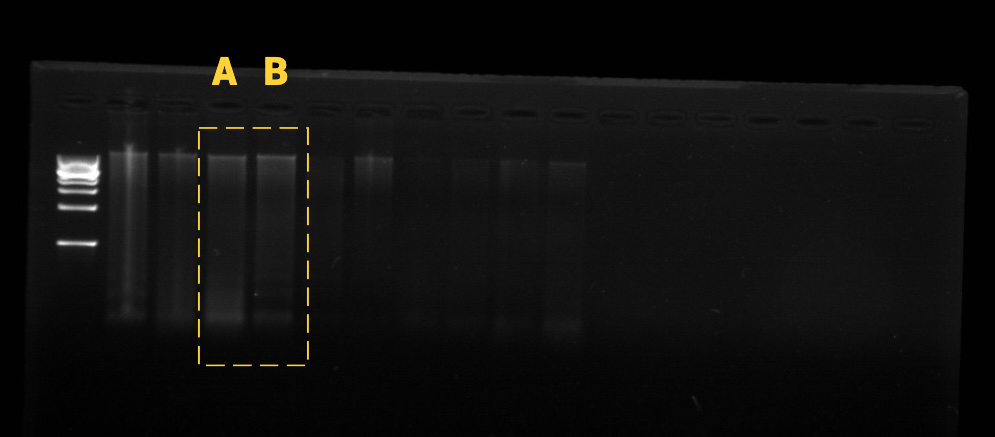
\includegraphics[width=0.75\linewidth]{Figures/20251010_DNA.jpg}
    \captionof{figure}{DNA原液电泳}
    \label{20251010_DNA}
\end{figure}

\subsection{PCR扩增引物设计}

\begin{table}[H]
    \centering
    \begin{tabular}{>{\raggedright\arraybackslash}p{1.5cm}>{\raggedright\arraybackslash}p{1.5cm}>{\raggedright\arraybackslash}p{6cm}>{\raggedright\arraybackslash}p{1.2cm}>{\raggedright\arraybackslash}p{1.2cm}>{\raggedright\arraybackslash}p{2cm}}
        \toprule
        \textbf{基因} & \textbf{位置} & \textbf{引物序列 (5'$\to$3')} & \textbf{T$_m$/\unit{\celsius}} & \textbf{GC\%} & \textbf{产物大小} \\
        \midrule
        \makecell[l]{\textit{ALDH2}} & \makecell[l]{1510} & \makecell[l]{F: TGGAGCCCAGTCACCCTTTGGT \\ R: atgggacagagcagaggctggg} & \makecell[l]{61.8 \\ 62.1} & \makecell[l]{59.1 \\ 63.6} & \makecell[l]{413} \\[12pt]
            
        \makecell[l]{\textit{TAS2R38}} & \makecell[l]{145} & \makecell[l]{F: TTTCTGCACTGGGTGGCAACCA \\ R: GCCGGCTGATGCTGAGACACAG} & \makecell[l]{61.2 \\ 62.1 } & \makecell[l]{54.5 \\ 63.6} & \makecell[l]{275} \\[12pt]
        
        \makecell[l]{\textit{TAS2R38}} & \makecell[l]{785/886} & \makecell[l]{F: TGCTCCTGCATCTGCACTGTCC \\ R: CATGCCCAGAGGGACAAGCTGC} & \makecell[l]{61.2 \\ 62.1} & \makecell[l]{59.1 \\ 63.6} & \makecell[l]{433} \\
            \bottomrule
    \end{tabular}
\end{table}

\subsection{PCR扩增}
第一次PCR产物电泳情况如图~\ref{20251017_PCR}，其中最左侧泳道为marker，最右侧为对照组（水），中间均为样品。所有样品泳道均无明显条带，只在末端产生微弱信号，说明PCR扩增失败。主要原因可能是实验所使用引物已变质分解，或在配置溶液过程中未控制好温度。
\begin{figure}[H] 
    \centering
    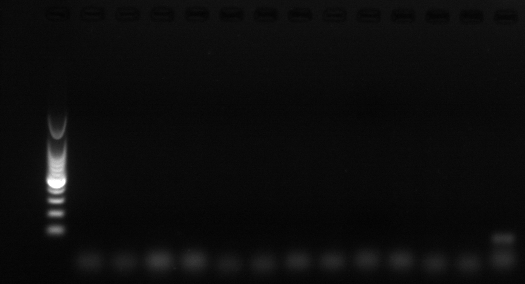
\includegraphics[width=0.75\linewidth]{Figures/20251017_PCR.jpg}
    \captionof{figure}{第一次PCR产物电泳}
    \label{20251017_PCR}
\end{figure}

第二次PCR产物电泳情况如图~\ref{20251025_PCR}，其中从左到右依次为marker，FA$\times$2，FTa$\times$2，FTb$\times$2，HA$\times$2，HTa$\times$2，HTb$\times$2，对照组（Label: 模版[\textbf{F}(eng)/\textbf{H}(an)]+引物[\textbf{A}(LDH2)/\textbf{T}(AS2R38)a/\textbf{T}(AS2R38)b]）。在更换引物后，所有样品泳道均产生了明显的条带，其中所有Tb引物泳道均产生了两条条带，推测上方条带是PCR产物，下方则为引物二聚体。
\begin{figure}[H] 
    \centering
    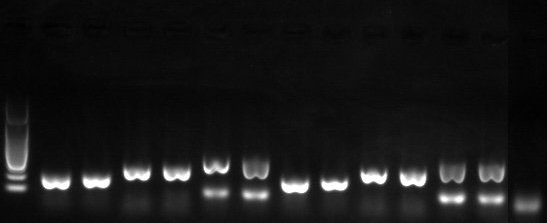
\includegraphics[width=0.75\linewidth]{Figures/20251025_PCR.jpg}
    \captionof{figure}{第二次PCR产物电泳}
    \label{20251025_PCR}
\end{figure}

\subsection{测序}
\subsubsection{样品1（冯）}
\begin{minipage}{0.20\textwidth}
    \centering
    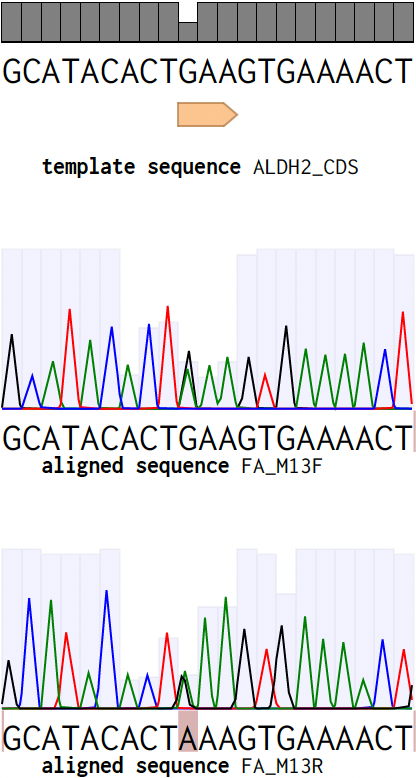
\includegraphics[width=\textwidth]{Figures/FA-1510.png}
    \captionof{figure}{FA-1510}
\end{minipage}
\hfill
\begin{minipage}{0.20\textwidth}
    \centering
    
\includegraphics[width=\textwidth]{Figures/FTa-145.png}
    \captionof{figure}{FTa-145}
\end{minipage}
\hfill
\begin{minipage}{0.20\textwidth}
    \centering
    
\includegraphics[width=\textwidth]{Figures/FTb-785.png}
    \captionof{figure}{FTb-785}
\end{minipage}
\hfill
\begin{minipage}{0.20\textwidth}
    \centering
    
\includegraphics[width=\textwidth]{Figures/FTb-886.png}
    \captionof{figure}{FTb-886}
\end{minipage}

\vspace{0.5cm}
使用Sanger法测序测得：
\begin{itemize}
    \item \textit{ALDH2} c.1510处G/A双峰 $\to$ \textbf{杂合子 G/A (rs671 GA)}
    \item \textit{TAS2R38} c.145处单C峰 $\to$ \textbf{野生型 C/C}
    \item \textit{TAS2R38} c.785处单C峰 $\to$ \textbf{野生型 C/C}
    \item \textit{TAS2R38} c.886处单G峰 $\to$ \textbf{野生型 G/G}
\end{itemize}

\subsubsection{样品2（韩）}
\begin{minipage}{0.20\textwidth}
    \centering
    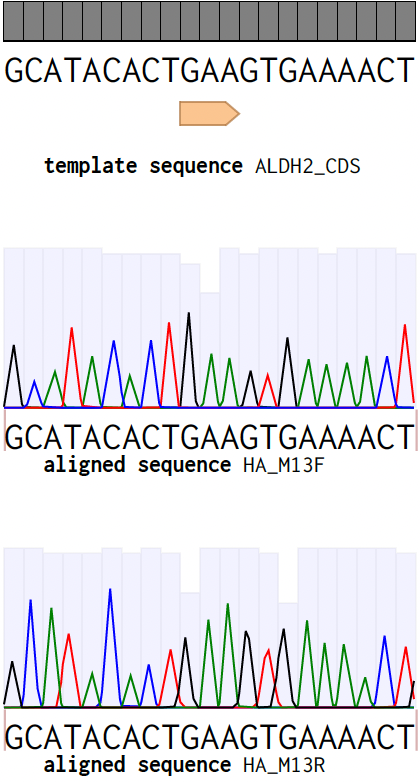
\includegraphics[width=\textwidth]{Figures/HA-1510.png}
    \captionof{figure}{FA-1510}
\end{minipage}
\hfill
\begin{minipage}{0.20\textwidth}
    \centering
    
\includegraphics[width=\textwidth]{Figures/HTa-145.png}
    \captionof{figure}{FTa-145}
\end{minipage}
\hfill
\begin{minipage}{0.20\textwidth}
    \centering
    
\includegraphics[width=\textwidth]{Figures/HTb-785.png}
    \captionof{figure}{FTb-785}
\end{minipage}
\hfill
\begin{minipage}{0.20\textwidth}
    \centering
    
\includegraphics[width=\textwidth]{Figures/HTb-886.png}
    \captionof{figure}{FTb-886}
\end{minipage}

\vspace{0.5cm}
使用Sanger法测序测得：
\begin{itemize}
    \item \textit{ALDH2} c.1510处单G峰 $\to$ \textbf{野生型 G/G}
    \item \textit{TAS2R38} c.145处单C峰 $\to$ \textbf{野生型 C/C}
    \item \textit{TAS2R38} c.785处单C峰 $\to$ \textbf{野生型 C/C}
    \item \textit{TAS2R38} c.886处单G峰 $\to$ \textbf{野生型 G/G}
\end{itemize}

\subsection{系统发生树}
选用23个物种的基因序列作系统发生树的样本（数据来源于UCSC Genome）：Human、Chimp、Gorilla、Gibbon、Green Monkey、Rhesus、Marmoset、Mouse Lemur、Mouse、Rat、Rabbit、Hedgehog、Pig、Cow、Sheep、Dolphin、Horse、Dog、Panda、Cat、Elephant、Armadillo，以及Tasmanian Devil作为外群。采用三种方法（NJ、MP、ML）建树，每次均进行1000次bootstrap，得到系统发生树如图~\ref{aldh2ml}-\ref{tas2r38-nj}。

\vspace{1cm}

\begin{minipage}[h]{0.49\textwidth}
    \centering
    
\includegraphics[width=\linewidth]{Figures/ALDH2_ML.png}
    \captionof{figure}{\textit{ALDH2}-ML}
    \label{aldh2ml}
\end{minipage}
\hfill
\begin{minipage}[h]{0.49\textwidth}
    \centering
    
\includegraphics[width=\linewidth]{Figures/ALDH2_MP.png}
    \captionof{figure}{\textit{ALDH2}-MP}
    \label{aldh2mp}
\end{minipage}

\vspace{0.5cm}

\begin{minipage}[h]{0.49\textwidth}
    \centering
    
\includegraphics[width=\linewidth]{Figures/ALDH2_NJ.png}
    \captionof{figure}{\textit{ALDH2}-NJ}
    \label{aldh2nj}
\end{minipage}
\hfill
\begin{minipage}[h]{0.49\textwidth}
    \centering
    
\includegraphics[width=\linewidth]{Figures/TAS2R38_ML.png}
    \captionof{figure}{\textit{TAS2R38}-ML}
    \label{tas2r38-ml}
\end{minipage}

\vspace{0.5cm}

\begin{minipage}[h]{0.49\textwidth}
    \centering
    
\includegraphics[width=\linewidth]{Figures/TAS2R38_MP.png}
    \captionof{figure}{\textit{TAS2R38}-MP}
    \label{tas2r38-mp}
\end{minipage}
\hfill
\begin{minipage}[h]{0.49\textwidth}
    \centering
    
\includegraphics[width=\linewidth]{Figures/TAS2R38_NJ.png}
    \captionof{figure}{\textit{TAS2R38}-NJ}
    \label{tas2r38-nj}
\end{minipage}

\section{讨论}
\subsection{基因型与表型对照}

\begin{table}[H]
    \centering
    \begin{tabular}{>{\raggedright\arraybackslash}p{1.5cm} >{\raggedright\arraybackslash}p{3cm} >{\raggedright\arraybackslash}p{3.5cm} >{\raggedright\arraybackslash}p{3cm} >{\raggedright\arraybackslash}p{3cm}}
        \toprule
        \textbf{受试者} & \textbf{位点} & \textbf{基因型} & \textbf{预测表型} & \textbf{实际表型} \\
        \midrule

        \multirow{4}{*}{张乐} 
        & \textit{ALDH2} c.1510 & G/G （野生型） & 乙醛代谢正常 & 饮酒无脸红反应 \\
        \cmidrule(lr){2-5}
        & \textit{TAS2R38} c.145 & C/G（杂合突变） & & \\
        & \textit{TAS2R38} c.785 & C/T（杂合突变） & 苦味不敏感 & 略感苦味 \\
        & \textit{TAS2R38} c.886 & G/A（杂合突变） & & \\

        \midrule

        \multirow{4}{*}{刘晋林} 
        & \textit{ALDH2} c.1510 & G/G （野生型） & 乙醛代谢正常 & 饮酒无脸红反应 \\
        \cmidrule(lr){2-5}
        & \textit{TAS2R38} c.145 & C/C（野生型） & & \\
        & \textit{TAS2R38} c.785 & C/C（野生型） & 苦味敏感 & 略感苦味 \\
        & \textit{TAS2R38} c.886 & G/G（野生型） & & \\

        \midrule

        \multirow{4}{*}{姜歆宇} 
        & \textit{ALDH2} c.1510 & G/A（杂合突变） & 乙醛代谢能力降低 & 不饮酒 \\
        \cmidrule(lr){2-5}
        & \textit{TAS2R38} c.145 & C/C（野生型） & & \\
        & \textit{TAS2R38} c.785 & C/C（野生型） & 苦味敏感 & 略感苦味 \\
        & \textit{TAS2R38} c.886 & G/G（野生型） & & \\

        \midrule

        \multirow{4}{*}{韩翔宇} 
        & \textit{ALDH2} c.1510 & G/G（野生型） & 乙醛代谢正常 & 不饮酒 \\
        \cmidrule(lr){2-5}
        & \textit{TAS2R38} c.145 & C/C（野生型） & & \\
        & \textit{TAS2R38} c.785 & C/C（野生型） & 苦味敏感 & 略感苦味 \\
        & \textit{TAS2R38} c.886 & G/G（野生型） & & \\

        \midrule

        \multirow{4}{*}{冯翊展} 
        & \textit{ALDH2} c.1510 & G/A（杂合突变） & 乙醛代谢能力降低 & 饮酒脸红 \\
        \cmidrule(lr){2-5}
        & \textit{TAS2R38} c.145 & C/C（野生型） & & \\
        & \textit{TAS2R38} c.785 & C/C（野生型） & 苦味敏感 & 略感苦味 \\
        & \textit{TAS2R38} c.886 & G/G（野生型） & & \\

        \bottomrule
    \end{tabular}
    \caption{五位受试者的 \textit{ALDH2} 与 \textit{TAS2R38} 基因型及其对应表型}
\end{table}

对比基因型与表型结果，我们发现五组样本中，\textit{ALDH2} 基因有三组表现出较为一致的基因型-表型对应关系，另有两组因缺乏饮酒行为而无法确定对应性；而 \textit{TAS2R38} 基因仅有一组样本的基因型与表型相符，其余四组则存在明显不一致。我们推测，\textit{TAS2R38} 基因型与表型不符的原因可能包括个体间对苦味感知阈值和主观认知的差异，同时实验中以口头描述作为苦味敏感程度判断依据，也可能引入一定的主观偏差与不确定性。

\subsection{\textit{ALDH2$^*$ 504Lys}的地理分布}
根据Li 等人的报道\citep{liRefinedGeographicDistribution2009a}，\textit{ALDH2$^*$ 504Lys}几乎仅存在于东亚地区，其中最高的等位基因频率出现在中国东南部人群中（可达 40.9\%）。在本实验中，我们检测到的五份样品中有两份携带该突变基因，且样本均来自中国东南地区（浙江与江西），这一观察结果与前述研究中关于突变地理分布的描述一致。

\begin{figure}[H]
    \centering
    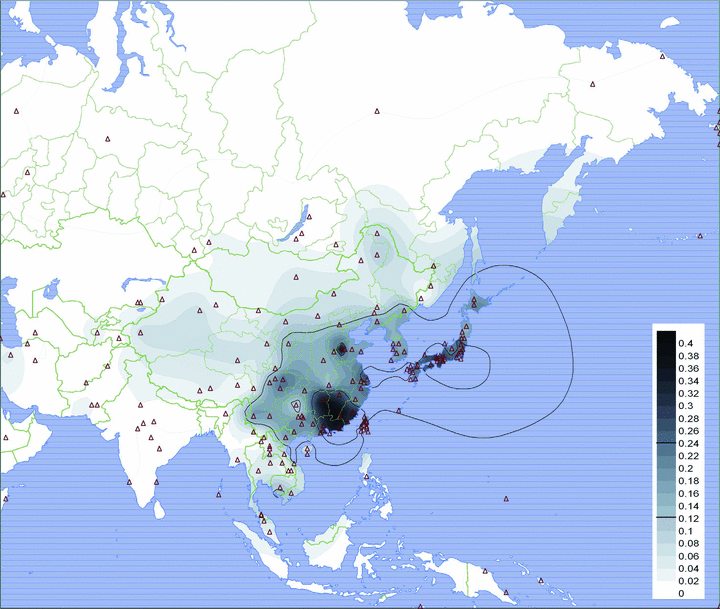
\includegraphics[width=0.9\linewidth]{Figures/ALDH2 504Lys Distribution.png}
    \captionof{figure}{\textit{ALDH2$^*$ 504Lys}分布}
\end{figure}

Li 等人（2009）进一步指出，尽管 \textit{ALDH2$^*$ 504Lys} 等位基因在中国东南部的频率最高，但其很可能起源于中国中部地区的古代汉族人群。在中国南方的土著族群（如苗瑶语系、侗台语系的侗族和拉珈族）以及台湾、海南的原住民中，该等位基因的频率极低或几乎缺失。历史与群体遗传学研究表明，现代中国东南部地区的突变群体主要是来自中国中部的迁徙者，突变频率的升高可能是在迁徙过程中由携带者群体传播并保留下来的。此外，历史上包括鲜卑、匈奴、契丹、女真等在内的阿尔泰语系族群曾迁入中国中部，而现代阿尔泰语系人群中该突变频率极低，因此他们的基因融入有可能在 \textit{ALDH2$^*$ 504Lys} 的起源地即中国中部造成频率的稀释。

\textit{ALDH2} 的功能缺陷不仅影响乙醇代谢，还与多种疾病密切相关。在心血管系统中，\textit{ALDH2} 是将硝酸甘油转化为一氧化氮（NO）的主要酶，因此该酶的突变会显著削弱个体对硝酸甘油的药理反应，成为心血管药物遗传学中的关键问题之一 \citep{liMitochondrialAldehydeDehydrogenase22006}。此外，大量研究表明，慢性酒精摄入者中多种癌症的发生率显著升高，包括食管癌、胃癌、肝癌及上呼吸消化道癌症等，这些部位中乙醇被酒精脱氢酶代谢产生的乙醛被认为是重要的致癌因子之一。对于\textit{ALDH2$^*$ 504Lys} 携带者而言，由于其乙醛清除能力降低，体内乙醛积聚更显著，因此其患癌风险亦随之升高 \citep{yokoyamaAlcoholAldehydeDehydrogenase2001}。




\section{致谢}

感谢罗述金老师精心设计本次实验，内容严谨且结构完整，并在口头报告过程中耐心倾听并给予中肯的批评与指导。感谢徐霄老师对实验原理深入浅出、生动有趣的讲解，增强了我们对系统发生学理论的理解。感谢王杜宸学长对实验流程、操作步骤及系统发生学基本原理的详细讲解，并在实验过程中给予及时的提醒与指导。感谢张乐、刘晋林、韩翔宇、姜歆宇四位同学在实验中的协作与交流，使实验过程更加顺利与充实。

\clearpage

\bibliographystyle{unsrt}
\bibliography{ref}


\end{document}